We are using Qt for Python(PySide2) for the NeXus Constructor's graphical user interface. These are the official bindings for Qt 5 C++ API, provided by the Qt company.
\bigskip
There are two main methods of using Qt in Python, the more common "Widgets" framework or Qt-Quick which uses a markup language called QML.
We are taking the Qt-Widgets approach to developing the NeXus constructor, as the tooling for Qt-Quick/QML seems to be a bit lacking and some of the bindings are not as pythonic, and rather use C++-like idioms. Widgets also look more native to the OS running them. The main advantage QML provides is it's scaling for high-resolution displays or mobile devices.
\bigskip
Since version 5.12 PySide2 has included the Qt3D module in Qt5. We are utilising this with our 3d View of components in the neutron experiments. Qt3D provides a high-level interface to OpenGL which allows us to display the geometry information of components as well as an animated pulsed neutron beam. Qt3D's entity framework is similar to other GUI frameworks and 3D engines, such as unity. This means all the textures, meshes and transformations can be stored with a single entity in the Qt3d view, which is convenient for easily changing aspects of the 3d object. 
\bigskip
\begin{figure}
\caption{Qt3D's element inspector}
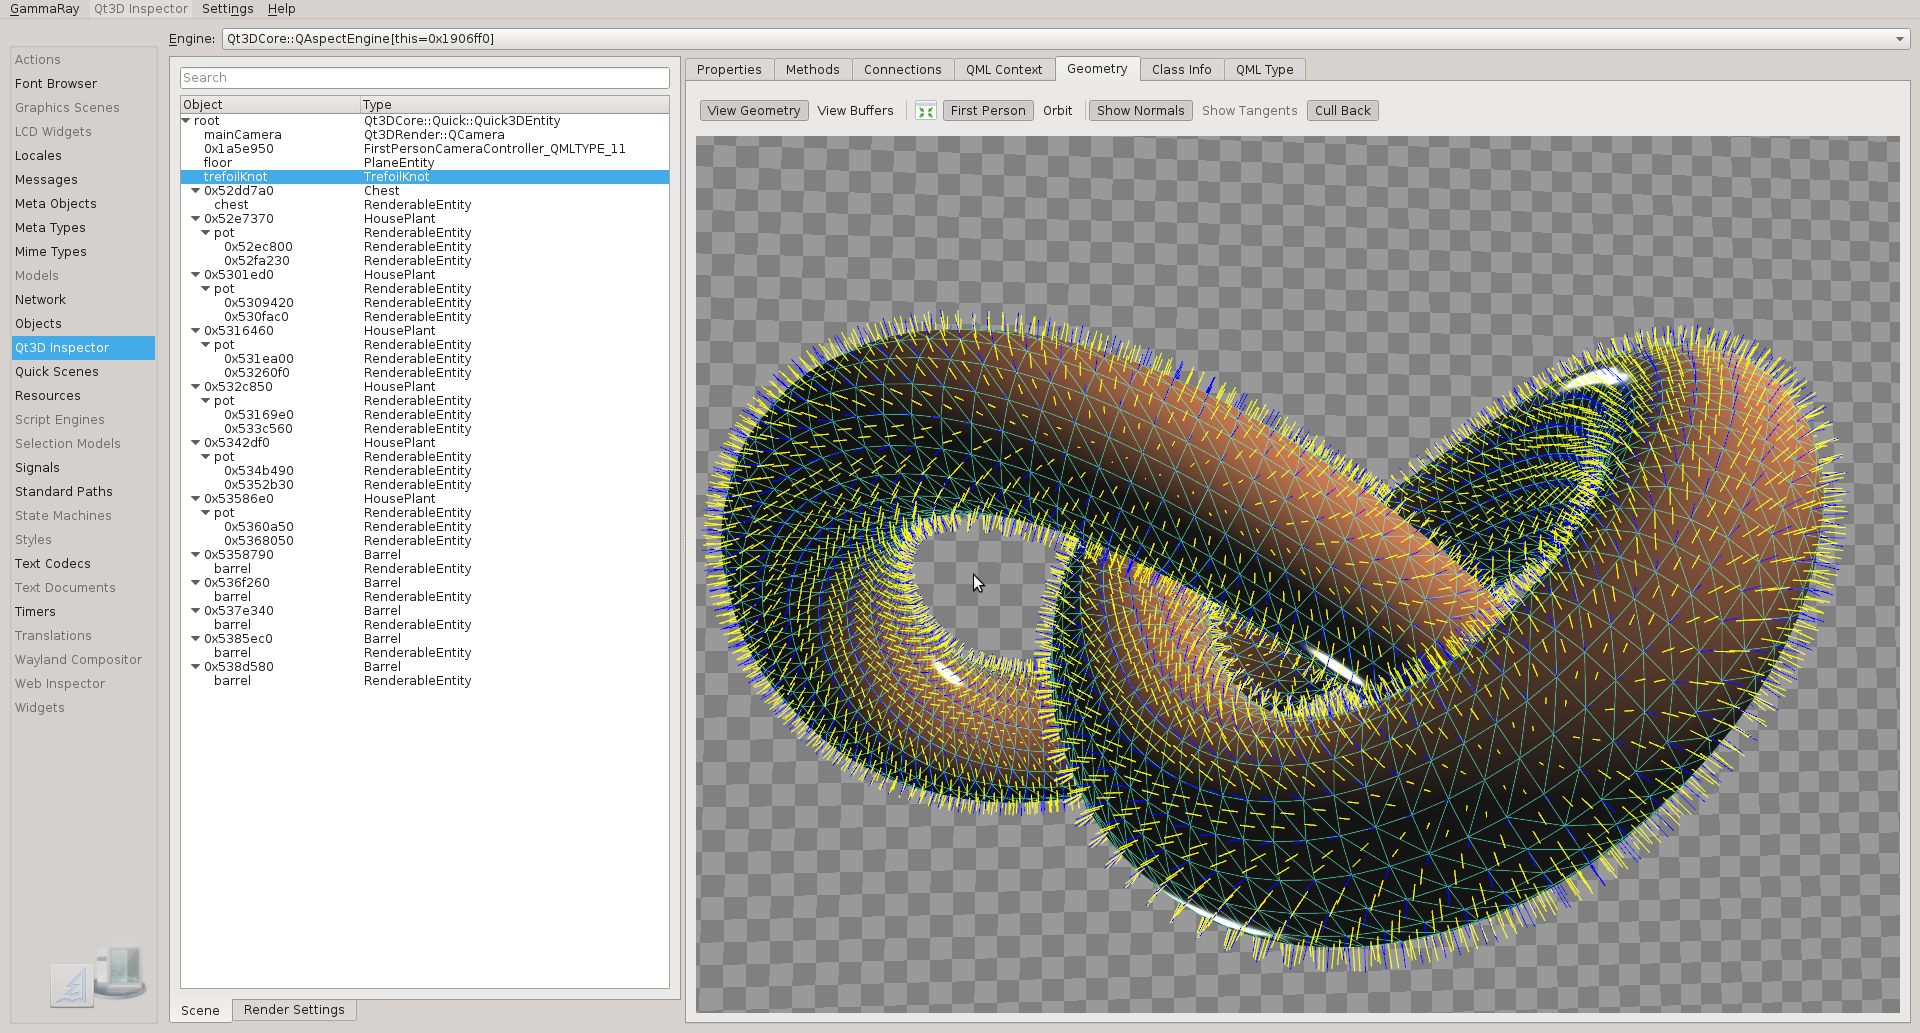
\includegraphics[width=\linewidth]{qt3d.png}
\end{figure}
\bigskip

The code snippet below shows the usage of a typical Qt3D view in python. Qt3D provides some high-level geometry types for adding cylinders, meshes, spheres as well as several other shapes. This is all wrapping OpenGL, and in the future Qt have stated they will support other graphics engines such as DirectX12, Vulkan and Metal. Currently there is some limited support for vulkan using the QVulkanWindow with a QVulkanInstance.

\begin{minted}[
frame=lines,
framesep=2mm,
fontsize=\footnotesize,
]
{python}
from PySide2.QtGui import QGuiApplication, QMatrix4x4, QQuaternion, QVector3D, QWindow
from PySide2.Qt3DCore import Qt3DCore
from PySide2.Qt3DRender import Qt3DRender
from PySide2.Qt3DExtras import Qt3DExtras

class CylinderWindow(Qt3DExtras.Qt3DWindow):
    def __init__(self):
        super(CylinderWindow, self).__init__()
        # Camera
        self.camera().lens().setPerspectiveProjection(45, 16 / 9, 0.1, 1000)
        # For camera controls
        self.createScene()
        self.cam_controller = Qt3DExtras.QOrbitCameraController(self.rootEntity)
        self.cam_controller.setCamera(self.camera())
        self.setRootEntity(self.rootEntity)
        self.cylinders = []
        self.meshes = []
        self.transforms = []

    def createScene(self):
        # Root entity
        self.rootEntity = Qt3DCore.QEntity()
        # Material
        self.material = Qt3DExtras.QPhongMaterial(self.rootEntity)

    def add_cylinder(self, radius, length, x, y, z, rings=10, slices=10):
        cylinder_entity = Qt3DCore.QEntity(self.rootEntity)
        # Using built in Qt cylinder Mesh
        cylinder_mesh = Qt3DExtras.Qcylinder_mesh()
        cylinder_mesh.setRadius(radius)
        cylinder_mesh.setLength(length)
        cylinder_mesh.setSlices(rings)
        cylinder_mesh.setRings(slices)
        # Add transforms to move the shape
        cylinder_transform = Qt3DCore.QTransform()
        cylinder_transform.setTranslation(QVector3D(x, y, z))
        # Add components to 3D entity
        cylinder_entity.addComponent(cylinder_mesh)
        cylinder_entity.addComponent(self.material)
        cylinder_entity.addComponent(cylinder_transform)
        # Add to list for easy access later        
        self.cylinders.append(cylinder_entity)
        self.meshes.append(cylinder_mesh)
        self.transforms.append(cylinder_transform)
\end{minted}

